\chapter{Speaker Verification Systems}
\label{ch:speaker-verification-systems}

%TODO remodelar, retirando tudo sobre Speaker IDENTIFICATION

The process of speaker verification lies on the field of pattern classification, with the speaker's speech signal as input for a classifier. The usage of this type of system is to determine if a claimed identity is true (user is classified as ``enrolled") or false (user is classified as ``imposter").

Differently from the speaker identification process, where the inputted speech is tested for all enrolled speakers and identified as the one with the highest score, in speaker verification only one speaker (the claimed identity) is tested. In order to perform a better comparison, a test against a model representing the other speakers is executed and the resulted score is compared with the score from the previous test, delivering a more reliable process.

\section{Utterance}

An \textbf{utterance} is a piece of speech produced by a speaker. It may be a word, a statement or any vocal sound. The terms \emph{utterance} and \emph{speech signal} sometimes are used interchangeably, but from herenow speech signal will be defined as an utterance recorded, digitalized and ready to be processed. An example is shown in \figureref{speech_signal}.

\begin{figure}[ht]
    \centering
    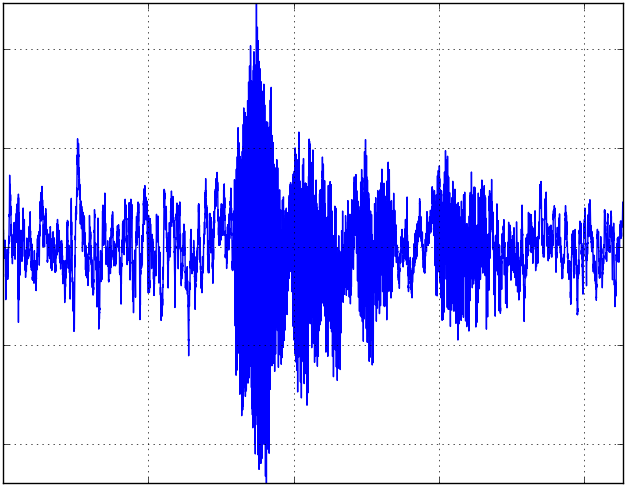
\includegraphics[width=\textwidth]{speech_signal}
    \caption{Speech signal from utterance ``karen livescu", \refbib{Woo, Park \& Hazen}{woo.park.hazen.2006}.}
    \label{fig:speech_signal}
\end{figure}

\section{Features}

The raw speech signal is unfit for use by an ASV. For a correct processing, the unique features from the speaker's vocal tract are extracted, what reduces the number of variables the system needs to deal with (leading to a simpler implementation) and performs a better evaluation (prevents the curse of dimensionality). Due to the stationary properties of the speech signal when analyzed in a short period of time, it is divided in overlapping frames of small and predefined length, to avoid ``loss of significancy", \refbib{Davis \& Mermelstein}{davis.mermelstein.1980}, \refbib{Rabiner \& Schafer}{rabiner.schafer.2007}. This extraction is executed by the MFCC algorithm, explained in details in \chapterref{feature-extraction}.

\section{Speaker Verification}
\label{sec:speaker-verification}

If a speaker $\mathcal{S}$ claims to be a particular user $\mathcal{S}_i$ from $\dvec{\mathcal{S}}$ (set of enrolled users), the strength of this claim resides on how similar the features $\dvec{X}$, extracted from a speech signal $\dvec{Y}$ spoken by $\mathcal{S}$, are to the features from $\mathcal{S}_i$ ``memorized" by the system. Then a simple equation

\begin{equation}
    \postpdf{\boldsymbol{X}}{\mathcal{S}_i} \verifytestB{\alpha}{\mathcal{S}}
    \label{eq:decision_speaker_verification}
\end{equation}

\noindent should be enough (considering all speakers equally probable). However, a subset of enrolled speakers may have vocal similarities or the features $\dvec{X}$ may be common to all enrolled users, leading to a misclassification of an imposter as a registered speaker (a false detection). To reduce the error rate the system must decide not only if a speech signal came from the claimed speaker, but also if it came from a set composed of all other enrolled speakers and compare the likelihoods.

\subsection{Likelihood Ratio Test}

Given the vector of features $\dvec{X}$, and assuming it was produced by only one speaker, the detection\footnote{the terms verification and detection are used interchangeably} task can be restated as a basic test between two hypoteses, \refbib{Reynolds}{reynolds.1995b}:

\begin{description}\itemsep0pt
    \item $H_0$: $\dvec{X}$ is from the claimed speaker $\mathcal{S}_i$;
    \item $H_1$: $\dvec{X}$ is \underline{not} from the claimed speaker $\mathcal{S}_i$.
\end{description}

\noindent The optimum test to decide which hypotesis is valid is the \textbf{likelihood ratio test} between both likelihoods $\postpdf{\dvec{X}}{H_0}$ and $\postpdf{\dvec{X}}{H_1}$, \refbib{Reynolds, Quatieri \& Dunn}{reynolds.quatieri.dunn.2000},

\begin{equation}
    \frac{\postpdf{\dvec{X}}{H_0}}{\postpdf{\dvec{X}}{H_1}} \verifytestB{\theta}{H_0}
    \label{eq:likelihood-ratio-test}
\end{equation}

\noindent where the decision threshold for accepting or rejecting $H_0$ is $\theta$ (a low $\theta$ generates a more permissive system, while a high $\theta$, a more restrictive). Applying the logarithm, the behavior of the likelihood ratio is maintained and \equationref{likelihood-ratio-test} is replaced by the \textbf{log-likelihood ratio}

\begin{equation}
    \Lambda(\dvec{X}) = \log \postpdf{\dvec{X}}{H_0} - \log \postpdf{\dvec{X}}{H_1}.
    \label{eq:log-likelihood-ratio-test}
\end{equation}

\subsection{Training}

Once the features are extracted from the speech signal, they are used to train the models $\lambda_{hyp}$ and $\lambda_{\overline{hyp}}$ for $H_0$ and $H_1$, respectively. A high-level demonstration of the training of $\lambda_{hyp}$ (mathematical representation of $\mathcal{S}_i$) is shown in \figureref{speaker-verification-training}:

\begin{figure}[ht]
    \centering
    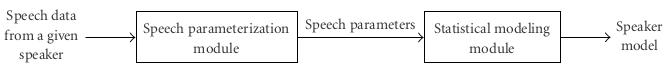
\includegraphics[width=\textwidth]{speaker-verification-training}
    \caption{The statistical model of $\mathcal{S}$ is created from the speech signal $\dvec{Y}$, \refbib{Bimbot et. al.}{bimbot.et.al.2004}.}
    \label{fig:speaker-verification-training}
\end{figure}

Due to $\lambda_{hyp}$ be a model of $\mathcal{S}_i$, the features used for training (i.e., estimate $p(\dvec{X}|\lambda_{hyp})$) are extracted from speech signals produced by $\mathcal{S}_i$. The model $\lambda_{\overline{hyp}}$, however, is not well-defined. It should be composed of the features extracted from speech signals from all other speakers except $\mathcal{S}_i$, but creating a single $\lambda_{\overline{hyp}}$ for each speaker is complicated and with no expressive gain. Instead, what is normally done is use all speakers to generate a background model $\lambda_{bkg}$, \refbib{Reynolds}{reynolds.1997}, in which the weight of each $\mathcal{S}_i$ is minimized.

\subsection{Test}

As seen in \equationref{likelihood-ratio-test}, the decision process is based on a function \emph{Score}. Replacing each $H_j$ for its corresponding model, the likelihood of a $\lambda_j$ given $\dvec{X}$ can be written as

\begin{equation}
    p(\dvec{X}|\lambda_j) = \prod_{t=1}^T p(\dvec{x}_t|\lambda_j).
    \label{eq:likelihood-prod}
\end{equation}

\noindent Using the logarithm function, \equationref{likelihood-prod} becomes

\begin{equation}
    \log p(\dvec{X}|\lambda_j) = \frac{1}{T} \sum_{t=1}^T \log p(\dvec{x}_t|\lambda_j),
    \label{eq:log-likelihood-sum}
\end{equation}

\noindent where the term $\frac{1}{T}$ is used to normalize the log-likelihood to the duration of the speech signal. That said, the likelihood ratio given by \equationref{log-likelihood-ratio-test} becomes

\begin{equation}
    \Lambda(\dvec{X}) = \log p(\dvec{X}|\lambda_{hyp}) - \log p(\dvec{X}|\lambda_{bkg}),
    \label{eq:score_of_X}
\end{equation}

\noindent and the speaker is accepted if $\Lambda(\dvec{X}) \geq \theta$, for an arbitrary value\footnote{$\theta$ is loosely used here. The proper equation would be $\Lambda(\dvec{X}) \geq \log\theta$.} of $\theta$ (see \figureref{likelihood_ratio_detector}).

\begin{figure}[ht]
    \centering
    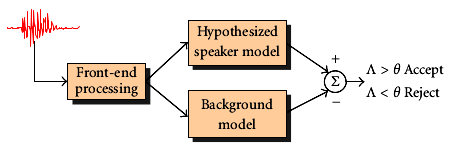
\includegraphics[width=0.75\textwidth]{likelihood-ratio-detector}
    \caption{Likelihood-ratio-based speaker verification system, \refbib{Bimbot et. al.}{bimbot.et.al.2004}.}
    \label{fig:likelihood_ratio_detector}
\end{figure}